\documentclass{article}

\usepackage{graphicx}
\usepackage{tikz}
\usepackage{tikzsymbols}
\usetikzlibrary{calc,patterns,shapes.geometric}
\pagestyle{empty}
\usepackage[margin=0pt]{geometry}
\geometry{papersize={14in,12in}}

\def\centerarc[#1](#2)(#3:#4:#5){\draw[#1] ($(#2)+({#5*cos(#3)},{#5*sin(#3)})$) arc (#3:#4:#5);}

\begin{document}
	\begin{figure}
		\centering
		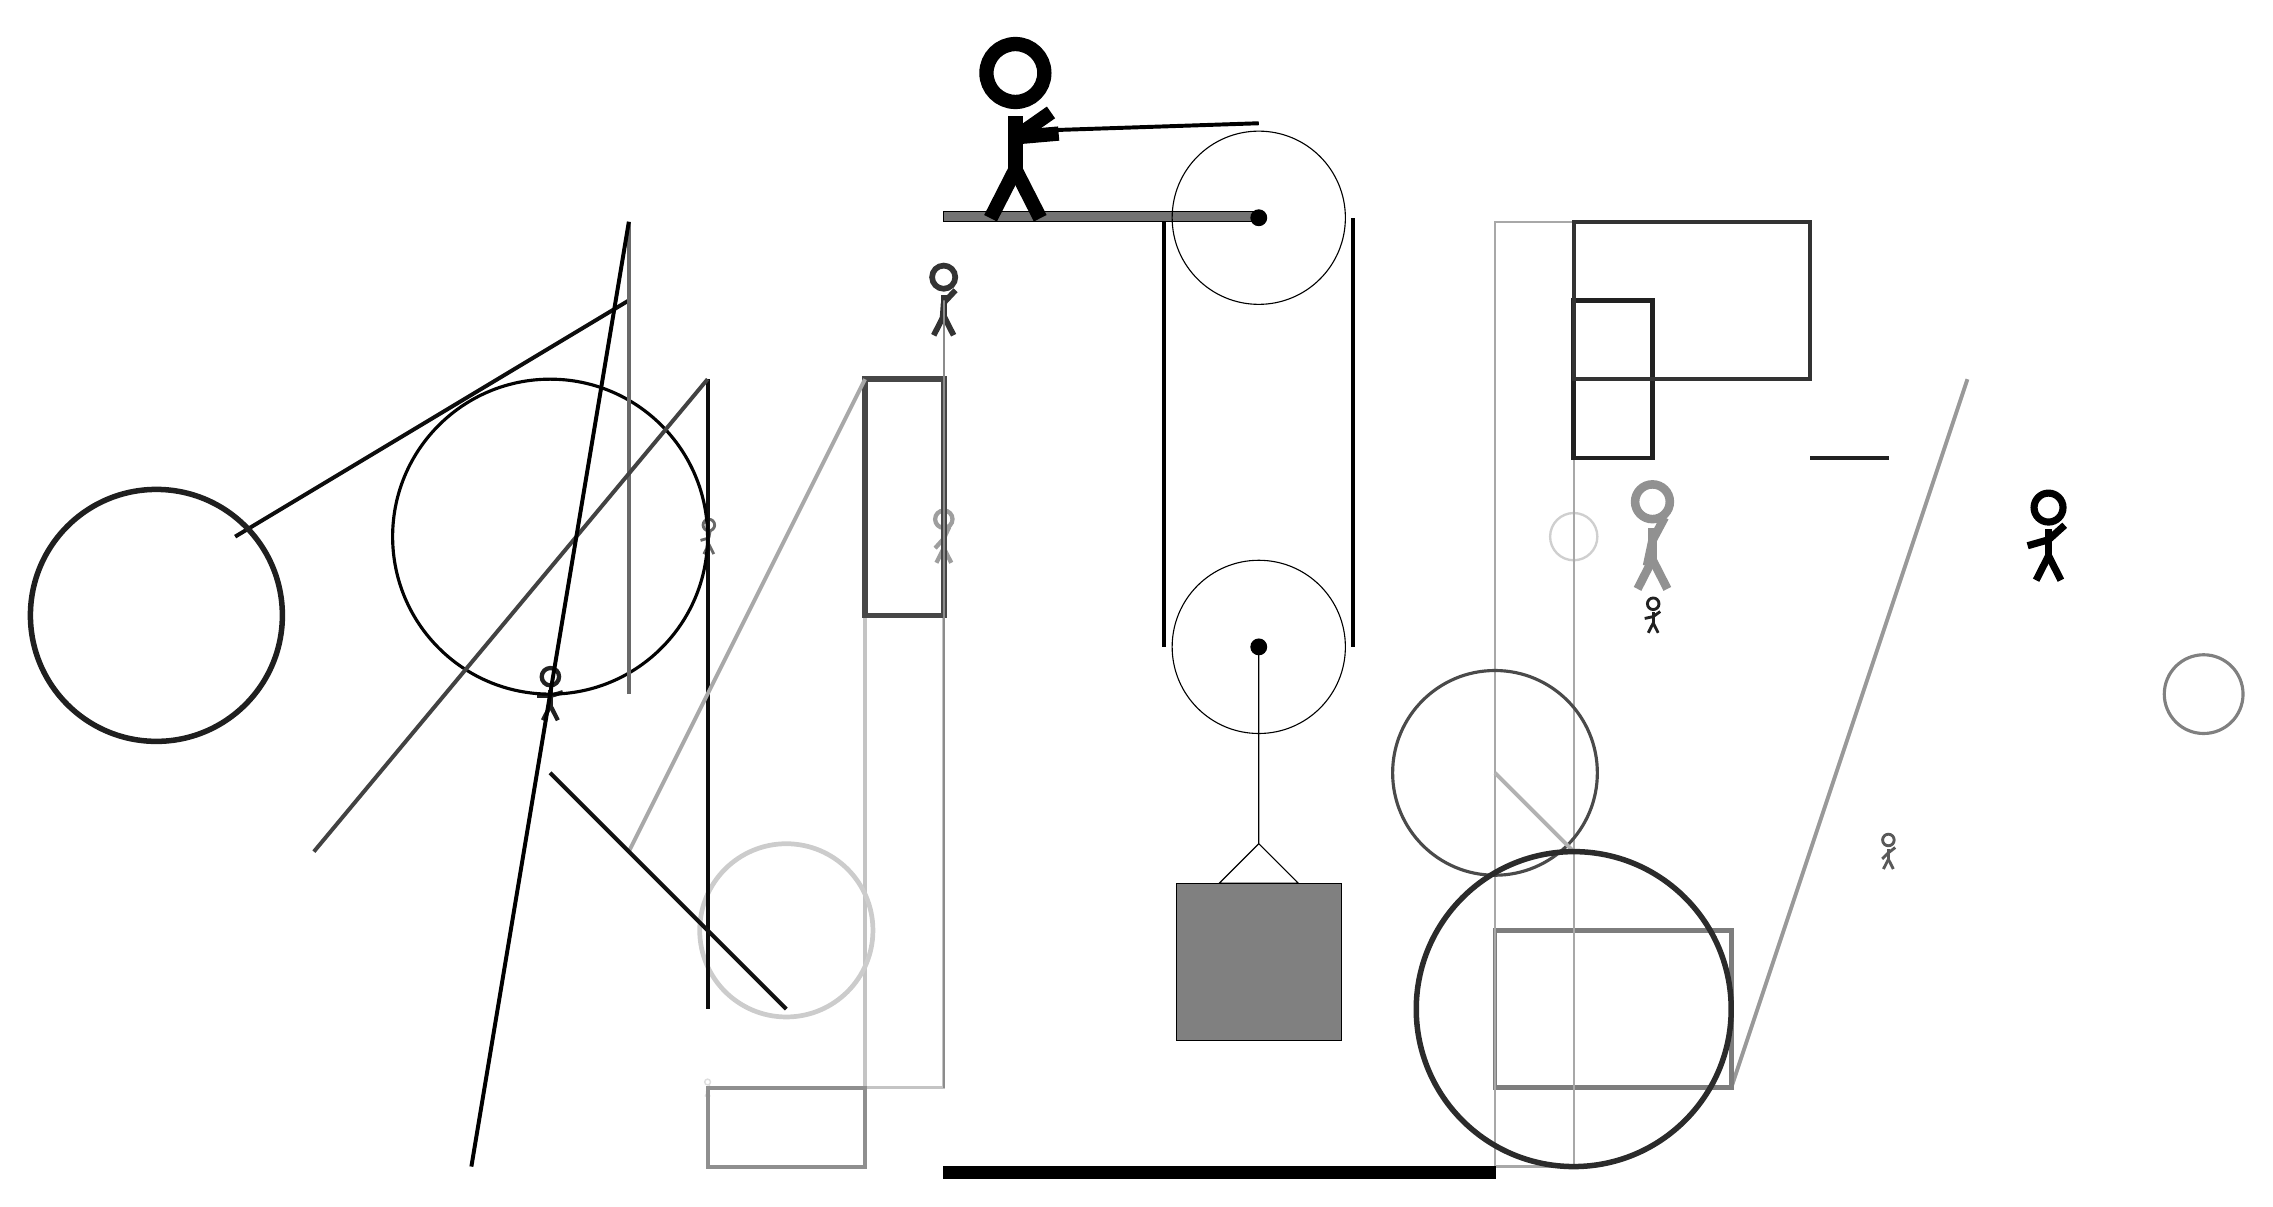
\begin{tikzpicture}
			%%%%% START %%%%%
			
			\draw[fill=black!55] (-2, 9) rectangle (2, 9.125);
			
			\draw (2, 3.6) circle (1.1);
			\draw[fill=black] (2, 3.6) circle (0.1);
			
			\draw (2, 9.05) circle (1.1);
			\draw[fill=black] (2, 9.05) circle (0.1);
			
			\draw[line width=0.5mm, color=black!40](8, -2) -- (11, 7);
			
			\node[line width=0.5mm, color=black!80] at (-2, 8) {\Strichmaxerl[4][86][47]};
			\node[line width=0.4mm, color=black!38] at (-2, 5) {\Strichmaxerl[3][48][65]};
			\draw [line width=0.2mm, color=black!42](-4, 7) circle (0.0);
			\draw [line width=0.3mm, color=black!19](6, 5) circle (0.3);
			\draw[line width=0.6mm, color=black!51] (5, -2) rectangle (8, 0);
			\draw[line width=0.3mm, color=black!34] (5, 9) rectangle (6, -3);
			
			\node[line width=0.4mm, color=black!43] at (7, 5) {\Strichmaxerl[6][78][62]};
			\draw[line width=0.4mm, color=black!23] (-3, 7) rectangle (-2, -2);
			\draw[line width=0.5mm, color=black!87](10, 6) -- (9, 6);
			\node[line width=0.4mm, color=black!87] at (-7, 3) {\Strichmaxerl[3][0][17]};
			\draw[line width=0.5mm, color=black!95](-6, 8) -- (-11, 5);
			\draw [line width=0.4mm, color=black!71](5, 2) circle (1.3);
			
			\node[line width=0.6mm, color=black!13] at (-5, -2) {\Strichmaxerl[1][72][60]};
			\draw[line width=0.7mm, color=black!72] (-3, 4) rectangle (-2, 7);
			\draw [line width=0.4mm, color=black!50](14, 3) circle (0.5);
			
			\node[line width=0.5mm, color=black!65] at (10, 1) {\Strichmaxerl[2][44][38]};
			
			\draw[line width=0.5mm, color=black!30](5, 2) -- (6, 1);
			\draw [line width=0.6mm, color=black!20](-4, 0) circle (1.1);
			\draw[line width=0.4mm, color=black!38] (5, 8) rectangle (5, 8);
			\node[line width=0.7mm, color=black!59] at (-5, 5) {\Strichmaxerl[2][17][80]};
			
			\draw[line width=0.5mm, color=black!44] (-3, -2) rectangle (-5, -3);
			
			\draw [line width=0.7mm, color=black!83](6, -1) circle (2.0);
			\draw[line width=0.5mm, color=black!95](-5, 7) -- (-5, -1);
			\draw [line width=0.4mm, color=black!99](-7, 5) circle (2.0);
			\draw[line width=0.6mm, color=black!87] (6, 8) rectangle (7, 6);
			\draw[line width=0.5mm, color=black!34](-3, 7) -- (-6, 1);
			\draw[line width=0.5mm, color=black!59](-6, 3) -- (-6, 9);
			\node[line width=0.7mm, color=black!87] at (7, 4) {\Strichmaxerl[2][12][36]};
			\draw[line width=0.5mm, color=black!93](-4, -1) -- (-7, 2);
			\draw[line width=0.5mm, color=black!74](-5, 7) -- (-10, 1);
			
			\draw[line width=0.5mm, color=black!80] (6, 7) rectangle (9, 9);
			\draw [line width=0.7mm, color=black!88](-12, 4) circle (1.6);
			\draw[line width=0.3mm, color=black!45] (-2, 8) rectangle (-2, -2);
			\draw[line width=0.5mm, color=black!100](-6, 9) -- (-8, -3);
			\node[line width=0.4mm, color=black!100] at (12, 5) {\Strichmaxerl[5][16][42]};
			
			\draw (2, 3.6) -- (2, 1.1) -- (1.5, 0.6) -- (2.5, 0.6) -- (2, 1.1);
			\draw[fill=black!50] (0.95, 0.6) rectangle (3.05, -1.4);
			
			\draw[line width=0.5mm] (0.8, 9) -- (0.8, 3.6);
			\centerarc[line width=0.5mm](2, 3.6)(180:360:1.2000000000000002);
			\draw[line width=0.5mm](3.2, 3.6) -- (3.2, 9.05);
			\centerarc[line width=0.5mm](2, 9.05)(0:90:1.2000000000000002);
			\draw[line width=0.5mm](2, 10.25) -- (-1, 10.15);
			
			\node at (-1, 10.15) {\Strichmaxerl[10][-175][35]};
			
			\draw[fill=black] (-2, -3) rectangle (5, -3.15);
			
			%%%%% END %%%%%
		\end{tikzpicture}
	\end{figure}	
\end{document}